\section{Experiment design}
\subsection{Defining five equivalence classes}
As with source code, in regular expressions, there are multiple ways to express the same semantic concept.
For example, the regex, \verb!`aa*'! matches an \verb!a! followed by zero or more \verb!a!'s, and is is equivalent to \verb!`a+'! , which matches one or more \verb!a!'s.
What is not clear is which representation,  \verb!`aa*'!  or  \verb!`a+'!, is preferred.
Preferences in regex refactorings could come from a number of sources, including which is easier to maintain, easier to understand, or better conforms to community standards, depending on the goals of the programmer.

In this work, we introduce possible refactorings in regular expressions by identifying equivalence classes of regex representations and transformations between the representations.
These equivalence classes provide options for how to represent double-bounds in repetitions (e.g., \verb!`a{1,2}'! or \verb!`a|aa'!), single-bounds in repetitions (e.g., \verb!`a{2}'! or \verb!`aa'!), lower bounds in repetitions (e.g., \verb!`a{2,}'! or \verb!`aaa*'!), character classes (e.g., \verb!`[0-9]'! or \verb!`[\d]'!), and literals (e.g., \verb!`\a'! or \verb!`\x07'!).
We suggest directions for the refactorings, for example, from \verb!`aa*'!  to  \verb!`a+'!, based on two high-level concepts: which representation appears most frequently in source code (conformance to community standards) and which is more understandable by programmers, based on comprehension tests completed by 180 study participants.
Our results identify preferred representations for four of the five equivalence classes based on mutual agreement between community standards and understandability, with three of those being statistically significant. For the fifth group on double-bounded repetitions, two recommendations are given depending on the goals of the programmer.

Our contributions are:
\begin{itemize}
\item Identification of  equivalence classes for regular expressions with possible transformations within each class,
\item Conducted an empirical study with 180 participants evaluating regex understandability,
\item Conducted an empirical study identifying opportunities for regex refactoring  in Python projects based on how regexes are expressed, and
\item {Identified preferred regex representations and refactorings that are the most understandable and conform best to community standards, backed by empirical evidence.}
\end{itemize}

To our knowledge, this is the first work to apply refactoring to regular expressions. Further, we approach the problem of identifying preferred regex representations by looking at thousands of regexes in Python projects and measuring the understandability of various regex representations using human participants. The rest of the paper describes
equivalence classes and possible refactorings as well as our two empirical studies, one using source code artifacts and another using human participants.

\begin{figure*}[tb]
\centering
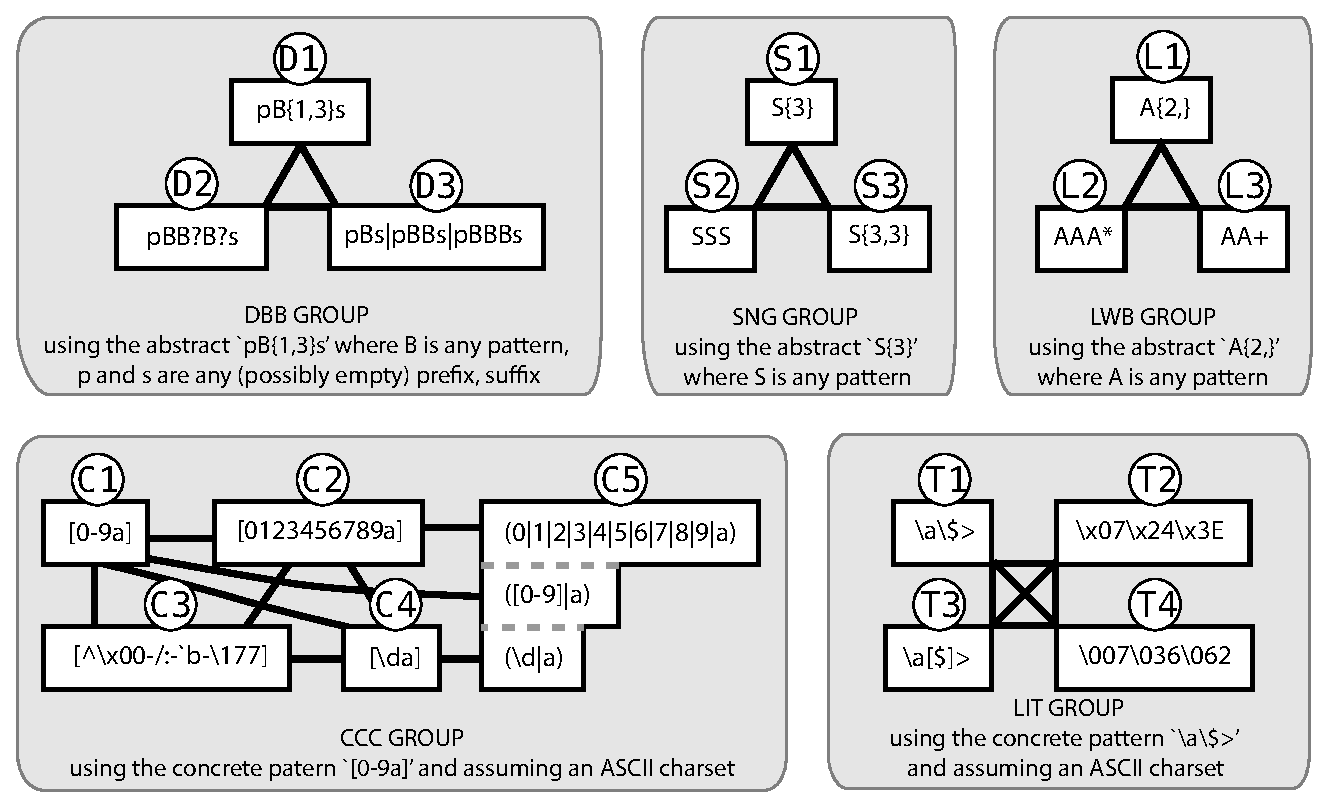
\includegraphics[width=\textwidth]{nontex/illustrations/refactoringTree.eps}
\vspace{-12pt}
\caption{Equivalence classes with various representations of semantically equivalent refactorings within each class. DBB = Double-Bounded, SNG = Single Bounded, LWB = Lower Bounded, CCC = Custom Character Class and LIT = Literal}
\vspace{-6pt}
\label{fig:refactoringTree}
\end{figure*}

After studying over 13,000 distinct regex strings from nearly 4,000 Python projects, we have defined a set of equivalence classes for regexes with refactorings that can transform among members in the classes.
For example,  \verb!AAA*! and \verb!AA+! are semantically identical, except one uses the star operator (indicating zero or more repetitions) and the other uses the plus operator (indicating one or more repetitions).
Both match strings with two or more \verb!A!'s.

Figure~\ref{fig:refactoringTree} displays the five equivalence classes in grey boxes and various semantically equivalent \emph{representations} of a regex are shown in white boxes. For example, LWB is an equivalence class with representations that all have a lower bound on repetitions. Regexes \verb!AAA*! and \verb!AA+!  are both members of this class mapping to representations L2 and L3, respectively, along with the L1 representation, \verb!A{2,}!.
The undirected edges between the representations define possible refactorings.
Identifying the best direction for each arrow in the possible refactorings is discussed in Section

We use concrete regexes in the representations to more clearly illustrate examples of the representations. However, the \verb!A!'s in the LWB group abstractly represent any pattern that could be operated on by a repetition modifier (literal characters, character classes, groups, etc.).   We chose the lower bound repetition threshold of  2 for illustration; in practice this could be any number, including zero.
Next, we describe each group, the representations, and possible transformations in detail:

\paragraph{CCC Group}
The Custom Character Class (CCC) group has regex representations that use the custom character class language feature or can be represented by such a feature.
A custom character class enables a programmer to specify a set of alternative characters, any of which can match.  For example, the regex \verb!`c[ao]t'! will match both the string ``cat" and the string ``cot" because, between the \verb!c! and \verb!t!, there is a custom character class, \verb![ao]!, that specifies either \verb!a! or \verb!o! (but not both) must be selected.  We use the term \emph{custom} to differentiate these classes created by the user from the default character classes, : \verb!\d!, \verb!\D!, \verb!\w!, \verb!\W!, \verb!\s!, \verb!\S! and \verb!.!,  provided by most regex libraries.
Next, we provide descriptions of each representation in this equivalence class:

\begin{description}  \itemsep -1pt
\item[C1:] Any pattern using a range feature like \verb![a-f]! as shorthand for all of the characters between `a' and `f' (inclusive) within a (non-negative) character class belongs to the C1 node.

\item[C2:] Any pattern that contains at least one (non-negative) custom character class  without any shorthand representations, specifically ranges or defaults. For example, \verb!`[012]'! is in C2, but \verb!`[0-2]'! is not.

\item[C3:] Any character classes expressed using negation, which is indicated by a caret (i.e., \verb!^!) followed by a custom character class specification.
For example, the pattern \verb![^ao]! matches every character \emph{except} \verb!a! or \verb!o!.  If the applicable character set is known (e.g., ASCII, UTF-8, etc.), then any non-negative character class can be represented as a negative character class.  For example, assuming an ASCII charset that has 128 characters: \verb!\x00-\x7f!, a character class representing the lower half: \verb![\x00-\x3f]! can be represented by negating the upper half: \verb![^\x40-\x7f]!.

\item[C4:] Any pattern using a default character class such as \verb!\d! or \verb!\W! within a (non-negative) character class belongs to the C4 node.

\item[C5:] While not expressed using a character class, these representations can be transformed into custom character classes by removing the ORs and adding square brackets (e.g., \verb!(\d|a)! in C5 is equivalent to \verb![\da]! in C4). All custom character classes expressed as an OR of length-one sequences, including defaults or other CCCs, are included in C5. Note that because an OR cannot be directly negated, it does not make sense to have an edge between C3 and C5 in Figure~\ref{fig:refactoringTree}, though C3 may be able to transition to C1, C2 or C4 first and then to C5.
\end{description}

A pattern can belong to multiple representations. For example,  \verb![a-f\d]! belongs to both C1 and C4.  The edge between C1 and C4 represents the opportunity to express the same pattern as \verb![a-f0-9]! by transforming the default digit character class into a range.  This transformed version would only belong to the C1 node.

\paragraph{DBB Group}
The Double-Bounded (DBB) group contains all regex patterns that use some repetition defined by a (non-equal) lower and upper boundary.  For example the pattern \verb!pB{1,3}s! represents a \verb!p! followed by one to three sequential \verb!B! patterns, then followed by a single \verb!s!.  This will match ``pBs", ``pBBs", and ``pBBBs".

\begin{description}  \itemsep -1pt
\item[D1:] Any pattern that  uses the curly brace repetition with a lower and upper bound, such as  \verb!pB{1,3}s!, belongs to the D1 node.
Note that  \verb!pB{1,3}s! can become \verb!pBB{0,2}s! by pulling the lower bound out of the curly braces and into the explicit sequence (or visa versa). Nonetheless, it would still be part of D1, though this within-node refactoring on D1 is not discussed in this work.
\item[D2:] Any pattern that uses the questionable (i.e., \verb!?!) modifier implies a lower-bound of zero and an upper-bound of one, and belongs to D2. For example, when a double-bounded regex has zero on the lower bound, as is the case with \verb!pBB{0,2}s!  in D1, transforming it to D2 involves replacing the curly braces with $n$ questionable modifiers, where $n$ is the upper bound,  creating \verb!pBB?B?s!.
\item[D3:] Any pattern that has a repetition with a lower and upper boundary and is expressed using ORs is part of D3.  The example, \verb!pB{1,3}s! would become \verb!pBs|pBBs|pBBs! by expanding on each option in the boundaries.
Note also that a pattern can belong to multiple nodes in the DBB group, for example, \verb!(a|aa)X?Y{2,4}! belongs to all three nodes.
\end{description}

Note that a pattern can belong to multiple nodes in the DBB group, for example, \verb!(a|aa)X?Y{2,4}! belongs to all three nodes: \verb!Y{2,4}! maps it to D1, \verb!X?!  maps it to D2, and \verb!(a|aa)!  maps it to D3.

\paragraph{LIT Group}
All patterns that are not purely default character classes have to use some literal tokens to specify what characters to match.  In Python and most other languages that support regex libraries, the programmer is able to specify literal tokens in a variety of ways.  In our example we use the ASCII charset, in which all characters can be expressed using hex and octal codes like \verb!\xF1!, and \verb!\0108!, respectively.  This group defines transformations among various representations of literals.

\begin{description}  \itemsep -1pt
\item[T1:] Patterns that do not use any hex characters (T2), wrapped characters (T3) or octal (T4), but use at least one literal character belong to the T1 node.
\item[T2:] Any pattern using hex tokens, such as \verb!\x07!, belongs to the T2 node.
\item[T3:]  Any literal wrapped in square brackets belongs to T3.
Literal character can be wrapped in brackets to form a custom character class of size one, such as \verb![x][y][z]!. This style is used most often to avoid using a backslash for a special character in the regex language, for example, \verb![{]! which must otherwise be escaped like \verb!\{!.

\item[T4:] Any pattern using octal tokens, such as \verb!\007!, belongs to the T4 node.
\end{description}

Patterns often fall in multiple of these representations, for example, \verb!abc\007! includes literals \verb!a!, \verb!b!, and \verb!c!, and also octal \verb!\007!, thus belonging to T1 and T4.

\paragraph{LWB Group}
The lower-bounded (LWB) group contains all patterns that specify only a lower boundary on the number of repetitions required for a match.  This can be expressed using curly braces with a comma after the lower bound but no upper bound, for example \verb!A{3,}! which will match `AAA', `AAAA', `AAAAA', and any number of A's greater or equal to 3.

\begin{description}  \itemsep -1pt
\item[L1:] Any pattern using this curly braces-style LWB repetition belongs to node L1.
\item[L2:] The kleene star (KLE) means zero-or-more of something, and so \verb!X*! is equivalent to \verb!X{0,}!.  Any pattern using KLE belongs to the L2 node.
\item[L3:] One of the most commonly used regex features is additional repetition (ADD), for example \verb!T+! which means one-or-more T's.  This is equivalent to \verb!T{1,}!.  Any pattern using ADD repetition belongs to the L3 node.
\end{description}

Regex patterns often belong to multiple nodes, for example, with \verb!A+B*!,  \verb!A+! maps it to L3 and \verb!B*! maps it to L2. We note that the refactorings from L1 to L3 and L2 to L3 are not always possible, specifically when the lower bound is zero and the pattern is not repeated in sequence (e.g., \verb!`A*'! or \verb!`A{0,}'!).

\paragraph{SNG Group} This equivalence class contains  three representations of a regex that  deal with repetition of a single element in the regex, represents by \verb!S!.

\begin{description}  \itemsep -1pt
\item[S1:] Any pattern with a single repetition boundary in curly braces belongs to S1. For example,   \verb!S{3}!, states that S appears exactly three times in sequence.
\item[S2:] Any pattern that is explicitly repeated two or more times and could use repetition operators is part of S2.
\item[S3:] Any pattern with a double-bound in which the upper and lower bounds are same belong to S3. For example, \verb!S{3,3}! states \verb!S! appears a minimum of 3 and maximum of 3 times.
\end{description}

The important factor distinguishing this group from DBB and LWB is that there is a single finite number of repetitions, rather than a bounded range on the number of repetitions (DBB) or a lower bound on the number of repetitions (LWB).

\paragraph{Example}
Regular expressions will often belong to many representations in the equivalence classes described here, and often multiple representations within an equivalence class.
Using an example from a Python project, the regex \verb!`[^ ]*\.[A-Z]{3}'! is a member of S1, L2, C1, C3, and T1. This is because \verb!`[^ ]'! maps it to C3, \verb!`[^ ]*'! maps it to L2, \verb!`[A-Z]'! maps it to C1, \verb!`\.'! maps it to T1, and \verb!`[A-Z]{3}'! maps it to S1.
As examples of refactorings, moving from S1 to S2 would be possible by replacing  \verb!`[A-Z]{3}'! with  \verb!`[A-Z][A-Z][A-Z]'! and moving from L2 to L1 would replace \verb!`[^ ]*'! with \verb!`[^ ]{0,}'!, resulting in a refactored regex of:  \verb!`[^ ]{0,}\.[A-Z][A-Z][A-Z]'!.

We define understandability two ways. Assuming that common programming practices are more understandable than uncommon practices, we explore the frequencies of each representation from Figure~\ref{fig:refactoringTree} using thousands of regexes scraped from Python projects.
\subsection{Implementation details}
The goal of this study is to understand how frequently each of the regex representations appears in source code. Based on the results, we identify preferred representations using popularity in source code.

\subsection{Artifacts}
Artifacts were same as those described in chapter 3: Features.\todoNow{Adjust this to smoothly reflect the previous chapter}

\subsection{Metrics}
% We measure community support by matching each regex in the corpus to the representations (nodes) in Figure~\ref{fig:refactoringTree} and counting the number of \emph{patterns} that contain the representation and the number of \emph{projects} that contain the representation.  A \emph{pattern} is extracted from a utilization, as shown in Figure~\ref{fig:exampleUsage}.
% Note that a regex can belong to multiple representations, and a regex can belong to multiple projects since we collapsed duplicates and only analyze the distinct regex patterns.

\subsection{Analysis}
To determine how many of the representations match patterns in the corpus, we performed an analysis using the PCRE parser and by representing the regexes as token streams, depending on the characteristics of the representation. Our analysis code is available on GitHub\footurl{https://github.com/softwarekitty/regex_readability_study}. Next, we describe the process in detail:

\subsubsection{Presence of a Feature}
For the representations that only require a particular feature to be present, such as the question-mark in D2, the features identified by the PCRE parser were used to decide membership of patterns in nodes.
These feature-requiring nodes are as follows: D1 requires double-bounded repetition with different bounds, D2 requires the question-mark repetition, S1 requires single-bounded repetition, S3 requires double-bounded repetition with the same bounds,  L1 requires a lower-bound repetition, L2 requires the kleene star (\verb!*!) repetition, L3 requires the add (\verb!+!) repetition, and C3 requires a negated custom character class.

\subsubsection{Features  and Pattern}
For some representations, the presence of a feature is not enough to determine membership.
However,  the presence of a feature and properties of the pattern can determine membership.

Identifying D3 requires an OR containing at least two entries - some sequence present in one entry repeated N times, and then the same sequence present in another entry repeated N+1 times.  This is a hard pattern to detect directly, but we identified candidates by looking for a sequence of N repeating groups with an OR-bar (ie. \verb!|!) next to them on one side (either side).  This produced a list of 113 candidates which we narrowed down manually to 10 actual members.

Identifying T2 requires a literal feature that matches the regex \verb!(\\x[a-f0-9A-F]{2})! which reliably identifies hex codes within a pattern.
Similarly T4 requires a literal feature and must match the regex \verb!((\\0\d*)|(\\\d{3}))! which is specific to Python-style octal, requiring either exactly three digits after a slash, or a zero and some other digits after a slash.  Only one false positive was identified which was actually the lower end of a hex range using the literal \verb!\0!.

Identifying T3 requires that a single literal character is wrapped in a custom character class (a member of T3 is always a member of C2).
 T1 requires that no characters are wrapped in brackets or are hex or octal characters, which actually matches over 91\% of the total patterns analyzed.

\subsubsection{Token Stream }
The following representations were identified by representing the regex patterns as a sequence of dot-delimited tokens.
Identifying S2 requires any element to be repeated at least twice. This element could be a character class, a literal, or a collection of things encapsulated in parentheses.
Identifying C1 requires that a non-negative character class contains a range.  Identifying C2 requires that there exists a custom character class that does not use ranges or defaults. Identifying C4 requires the presence of a default character class within a custom character class, specifically, \verb!\d!, \verb!\D!, \verb!\w!, \verb!\W!, \verb!\s!, \verb!\S! and \verb!.!.  Identifying C5 requires an OR of length-one sequences (literal characters or any character class).
